%!TEX program = xelatex
\documentclass{article}
\usepackage{booktabs,longtable}
\usepackage{listings}
\usepackage[usenames,dvipsnames]{xcolor}
\usepackage{paralist}
% langugae defination
\lstdefinelanguage{Stata}{
    % Left for users to add missing commands,
    % with possibility of choosing different style.
    morekeywords={},
    % Popular add-on commands
    morekeywords=[2]{cntrade, chinafin, wbopendata, spmap},
    % System commands
    morekeywords=[3]{regress, summarize,sum,
                     display,log,tabstat,histogram,stem,graph,kdensity,box,rnormal, runiform,mean,sd,p5,p10,p15,p20,p25,p30,p35,p40,p45,p50,p55,p60,p65,p70,p75,p80,p85,p90,p95,p100,n,insheet,infile,infix,input,import,describe,compress,save,use,count,list,memory,str10,str8,excel,end,view,matrix,pwcorr,correlate,tab,display,lookfor,labelbook,codebook,sort,tabulate,table,label,order,encode,rename,notes,generate,gen,egen,recode,std,tab1,scatter,rowmean,colmean,keep,drop,append,merge,ttest,anova,margins,marginsplot,predict,pnorm,qnorm,rvfplot,test,logit,tobit,signtest,signrank,ranksum,kwallis,logistic,testparm},
    % Programming Key
    morekeywords=[4]{forvalues, if, foreach, set, using, in, cd, dir, ls,variable,define,values,data,pwd,close,},
    % Options Key
    morekeywords=[5]{by,over,stat,
                     text,replace,force,detail,normal,lines,width,jitter,start,clear,sheet,firstrow,half,row,column,col,normal,obs,noobs,nolabel,or,coef,all,expected,unequal,asbalanced,robust,clear},
    morecomment=[l]{//},
    % morecomment=[l]{*},  % `*` maybe used as multiply operator. So use `//` as line comment.
    morecomment=[s]{/*}{*/},
    % morecomment=[s]{,}{//},
    % The following is used by macros, like `lags'.
    morecomment=[n][keywordstyle9]{`}{'},
    morestring=[b]",
    sensitive=true,
    numbers=left, numberstyle=\tiny, stepnumber=1, numbersep=5pt,
}

\lstdefinestyle{numbers}{
    numbers=left,
    stepnumber=1,
    numberstyle=\tiny,
    xleftmargin=2em,
}
\lstdefinestyle{nonumbers}{
    numbers=none,
}
\lstdefinestyle{stata-plain}{
    % comment slanted and keywords bolded.
    language=Stata,
    basicstyle=\setmonofont{Consolas}\footnotesize\ttfamily,
}

\definecolor{darkgreen}{rgb}{0.0, 0.44, 0.0}
\definecolor{darkblue}{rgb}{0.0, 0.0, 0.55}
\definecolor{mahogany}{rgb}{0.75, 0.25, 0.0}
\definecolor{richcarmine}{rgb}{0.84, 0.0, 0.25}

\lstdefinestyle{stata-editor}{
    language=Stata,
    % size of the fonts for the code
    basicstyle=\setmonofont{Consolas}\footnotesize\ttfamily,
    % Color settings to match do-file editor style
    % Commands that are not included in the defination
    keywordstyle={\color{darkblue}},
    % Popular add-on commands
    keywordstyle=[2]{\color{darkblue}},
    % System commands
    keywordstyle=[3]{\color{darkblue}},
    % Keywords
    keywordstyle=[4]{\color{magenta}},
    % Built-in functions like rnormal
    keywordstyle=[5]{\color{mahogany}},
    % Used by macros, i.e. `lags'
    keywordstyle=[9]{\color{TealBlue}},
    stringstyle=\color{richcarmine},
    commentstyle=\color{darkgreen},
}


\lstset{
    language=Stata,
    style=stata-editor,
    % style=stata-editor,
    style=numbers,
    showstringspaces=false,
    breaklines,
    frame=single,
    % To add missing commands
    % morekeywords={xtreg, xtunitroot},
}


\usepackage{xcolor}
\usepackage{hyperref}
\usepackage{graphicx}
\usepackage{geometry}
\geometry{
            a4paper,
            left=27mm,  %% or inner=23mm
            right=27mm, %% or outer=18mm
            top=25.4mm, bottom=25.4mm,
            headheight=2.17cm,
            headsep=4mm,
            footskip=12mm
}

\hypersetup{
            breaklinks,
                   unicode,
            bookmarksnumbered=true,
            bookmarksopen=true,
            colorlinks,
            urlcolor=darkblue,
            citecolor=magenta,
            linkcolor=darkgreen,
            plainpages=false,
            pdfstartview=FitH,
            pdfborder={0 0 0},
            linktocpage
}

\usepackage[no-math,cm-default]{fontspec}
\defaultfontfeatures{Mapping=tex-text}
\RequirePackage{xunicode}
\RequirePackage{xltxtra}
\setmainfont[Ligatures=TeX]{Adobe Garamond Pro} %  (\textrm)
\setsansfont{Myriad Pro} %  (\textsf)
\setmonofont{Monaco}%Palatino Linotype
%-中文字体设置-%
\usepackage{xeCJK}
\setCJKmainfont[BoldFont={方正黑体简体},ItalicFont={方正楷体简体}]{方正书宋简体}
%方正书宋_GBK Adobe Song Std L华文中宋
\setCJKsansfont[BoldFont={方正黑体简体},ItalicFont={方正楷体简体}]{方正中等线简体}
\setCJKmonofont{微软雅黑Monaco}
\XeTeXlinebreaklocale "zh"
\XeTeXlinebreakskip = 0pt plus 1pt
\newfontfamily\gara{Adobe Garamond Pro}
\linespread{1.3}
\title{\bfseries{\color{blue}Stata} {\color{magenta}Class Notes}}
\author{\Large\gara\itshape{{\color{blue}E}than {\color{magenta}D}eng} \\ Version 1.0}


\begin{document}
\maketitle
\noindent\textbf{NOTES}: All the notes are from the website \href{http://www.ats.ucla.edu/stat/stata/notes/default13.htm}{UCLA Stata Class Notes}! The latest version of this notes (Highlighted PDF format) can be found on \href{http://ddswhu.com/}{EthanDeng\rq{}s Page}.

Stata is a powerful and yet easy-to-use statistical package that runs on Windows, Macintosh and Unix platforms.  This class is designed for people who are just getting started using Stata.  The students in the class will have a hands-on experience using Stata for statistics, graphics and data management.  The class notes are the scripts for the class available to the students in the class and to others on the Internet.  The Stata class notes do not contain any of the output.  The class notes are not meant to be a Stata textbook or a reference manual.  However, it is possible for individuals to use the class notes to help in learning Stata even if they don't enroll in the class.

\section{Entering Data}
\subsection{Stata Commands in this section}
The Stata commands in this section is list in Table \ref{tab:cmds in section 1}.
% Table generated by Excel2LaTeX from sheet 'Sheet1'
\begin{table}[htbp]
  \centering
  \caption{Stata commands in section: Entering Data\label{tab:cmds in section 1}}%
  \vskip 1ex
    \begin{tabular}{ll}
    \toprule
    Command & Explanation of Command \\
    \midrule
    \lstinline{cd} & Change directory \\
    \lstinline{dir} or \lstinline{ls} & Show files in current directory \\
    \lstinline{insheet} & Read ASCII (text) data created by a spreadsheet \\
    \lstinline{infile} & Read unformatted ASCII (text) data \\
    \lstinline{infix} & Read ASCII (text) data in fixed format \\
    \lstinline{input} & Enter data from keyboard \\
    \lstinline{import excel} & Import Excel .xls or .xlsx file \\
    \lstinline{describe} & Describe contents of data in memory or on disk \\
    \lstinline{compress} & Compress data in memory \\
    \lstinline{save} & Store the dataset currently in memory on disk in Stata data format \\
    \lstinline{use} & Load a Stata-format dataset \\
    \lstinline{count} & Show the number of observations \\
    \lstinline{list} & List values of variables \\
    \lstinline{clear} & Clear the entire dataset and everything else \\
    \lstinline{memory} & Display a report on memory usage \\
    \lstinline{set memory} & Set the size of memory \\
    \bottomrule
    \end{tabular}%
\end{table}%

\subsection{Demonstration and explanation}
\subsubsection{Comma-separated file with variable names}
We will start with inputting a spreadsheet type of data file into Stata. A spreadsheet type of file is created by programs such as Excel. For example, in Excel, we can save a file into a comma-separated-values format (\lstinline{.csv}) file. Stata reads in this type of data using the \lstinline{insheet} command. Let's first get to the directory where the file \lstinline{hs0.csv} is. This data file has variable names on the first line.

Here is a partial listing from the comma-separated file:
\begin{lstlisting}
gender,id,race,ses,schtyp,prgtype,read,write,math,science,socst
0,70,4,1,1,general,57,52,41,47,57
1,121,4,2,1,vocati,68,59,53,63,61
0,86,4,3,1,general,44,33,54,58,31
0,141,4,3,1,vocati,63,44,47,53,56
0,172,4,2,1,academic,47,52,57,53,61
0,113,4,2,1,academic,44,52,51,63,61
0,50,3,2,1,general,50,59,42,53,61
0,11,1,2,1,academic,34,46,45,39,36
0,84,4,2,1,general,63,57,54,,51
0,48,3,2,1,academic,57,55,52,50,51
\end{lstlisting}

And here are the Stata commands to read these data.
\begin{lstlisting}
cd d:\stata_data  /* note: directory and path may differ on your computer */
dir
insheet using hs0.csv, clear
describe
\end{lstlisting}
\subsubsection{Comma-separated file without variable names}
What if the data file does not have the variable names on the first line? We have a such file called \lstinline{hs0_noname.csv}.  We will also do a count to see if the inputting was successful.

\begin{lstlisting}
insheet gender id race ses schtyp prgtype read write math science socst using hs0_noname.csv, clear
count
\end{lstlisting}

\subsubsection{Space-delimited file}
To read a space-delimited file we will use \lstinline{infile} command. The first part of the file \lstinline{hs0.raw} is shown below.
\begin{lstlisting}
0 70 4 1 1 general 57 52 41 47 57
1 121 4 2 1 vocati 68 59 53 63 61
0 86 4 3 1 general 44 33 54 58 31
0 141 4 3 1 vocati 63 44 47 53 56
0 172 4 2 1 academic 47 52 57 53 61
0 113 4 2 1 academic 44 52 51 63 61
0 50 3 2 1 general 50 59 42 53 61
0 11 1 2 1 academic 34 46 45 39 36
0 84 4 2 1 general 63 57 54 . 51
0 48 3 2 1 academic 57 55 52 50 51
0 75 4 2 1 vocati 60 46 51 53 61
0 60 5 2 1 academic 57 65 51 63 61
\end{lstlisting}

Notice how we specify a character variable below.  The variable \textit{prgtype} is a string variable. We tell Stata that \textit{prgtype} is a string variable which should have a length of 10 by typing \lstinline{str10} \textbf{before} the variable name. We will use the \lstinline{hs0.raw} data file.

\begin{lstlisting}
infile gender id race ses schtyp str10 prgtype read write math science socst using hs0.raw, clear
\end{lstlisting}

\subsubsection{Fixed format file}

The other type of commonly used ASCII data format is fixed format. It always requires a codebook to specify which column(s) corresponds to which variable. Here is small example of this type of data with a codebook. Notice how we make use of the codebook in the \lstinline{infix} command below. We will use the \lstinline{schdat.fix} data file.

\begin{lstlisting}
 195  094951
 26386161941
 38780081841
 479700  870
 56878163690
 66487182960
 786  069  0
 88194193921
 98979090781
107868180801
\end{lstlisting}

% Table generated by Excel2LaTeX from sheet 'Sheet1'
\begin{table}[htbp]
  \caption{Codebook of the fix width dataset\label{tab:codebook of fix width}}
  \vskip 1ex
  \centering
    \begin{tabular}{cc}
    \toprule
    variable name & column number \\
    \midrule
    id    & 1-2 \\
    a1    & 3-4 \\
    t1    & 5-6 \\
    gender & 7 \\
    a2    & 8-9 \\
    t2    & 10-11 \\
    tgender & 12 \\
    \bottomrule
    \end{tabular}%
\end{table}%

\begin{lstlisting}
clear
infix id 1-2 a1 3-4 t1 5-6 gender 7 a2 8-9 t2 10-11 tgender 12 using schdat.fix
\end{lstlisting}

\subsubsection{Excel file}
The \lstinline{import excel} command was introduce in Stata 12. Here is what the file \lstinline{hsbdemo.xlsx} looks like.

\begin{figure}[htbp]
\centering
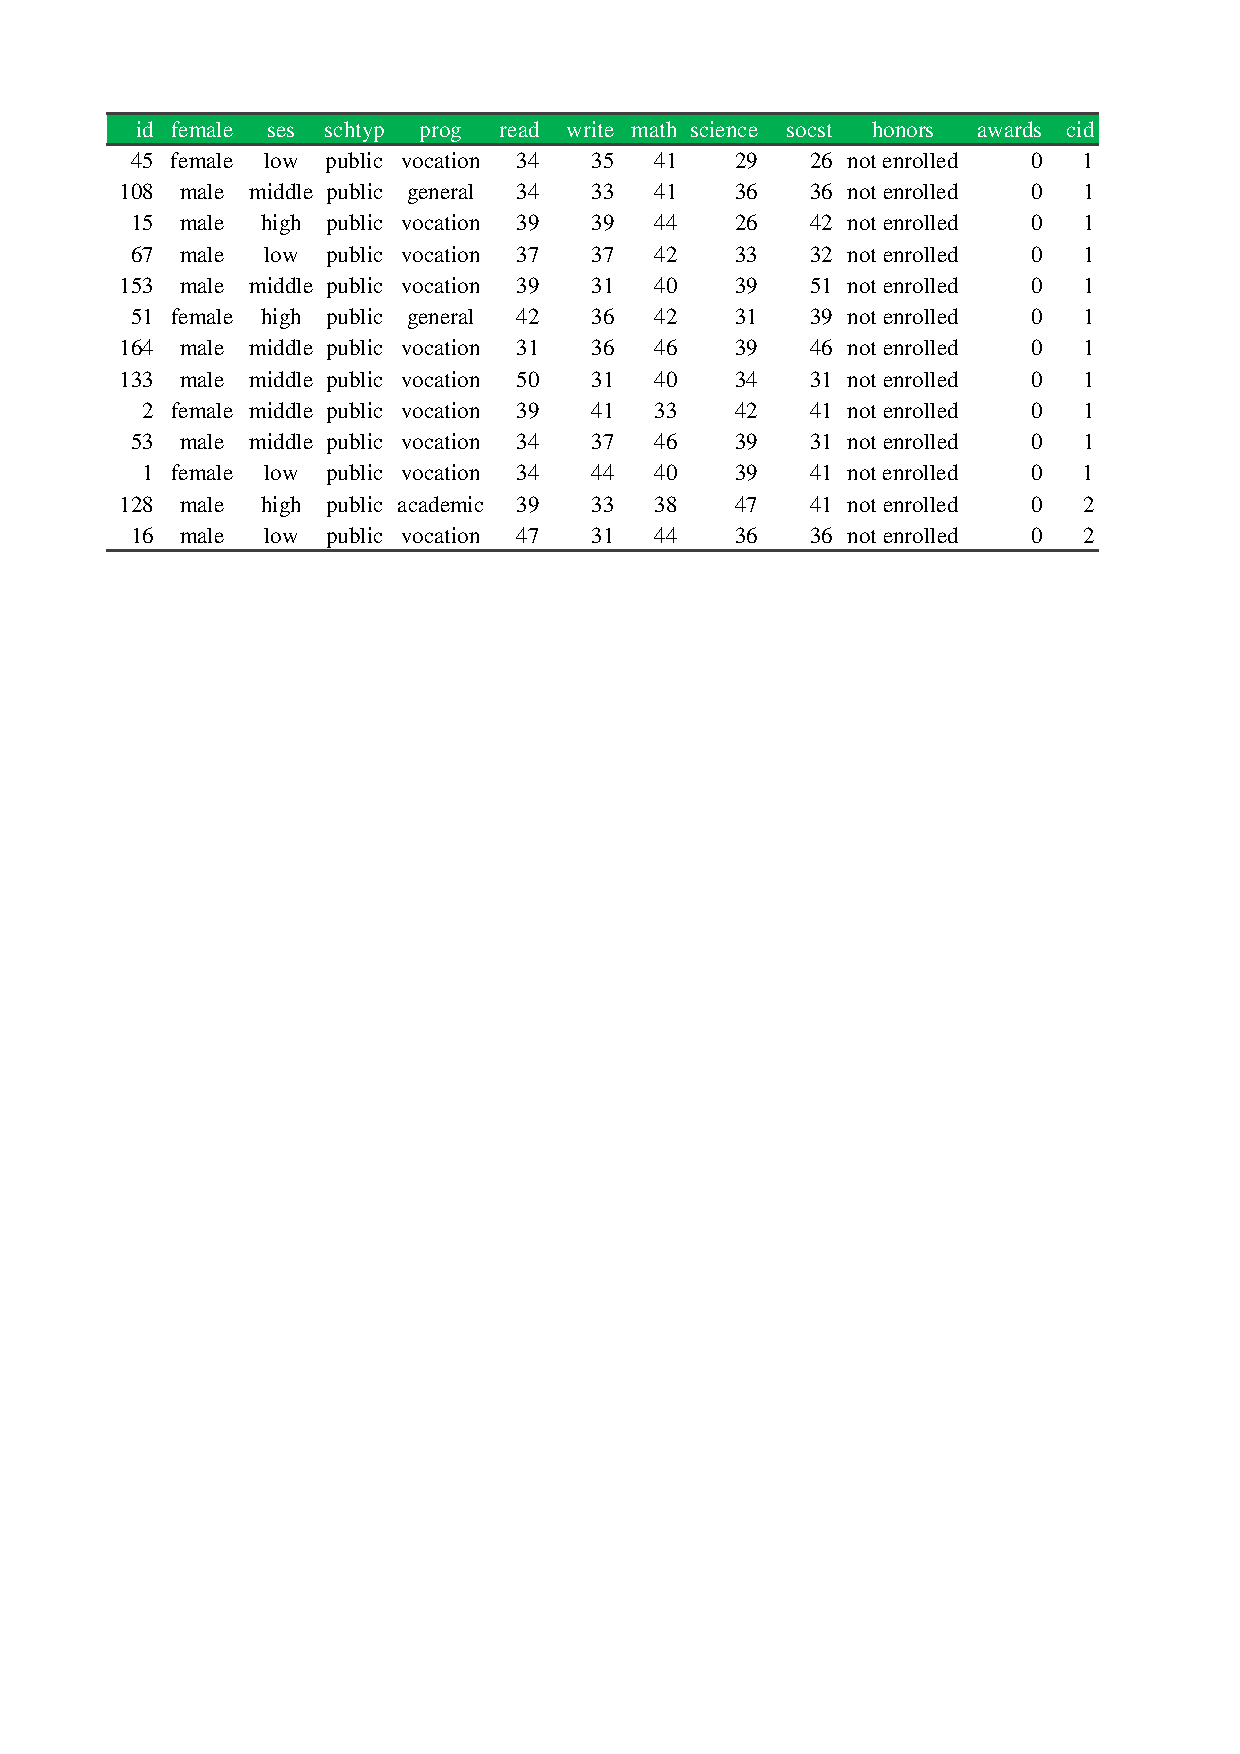
\includegraphics[width=0.85\textwidth]{hsbdemo.pdf}
\caption{Excel datasets sample}
\end{figure}

Here is how the spreadsheet is read in.

\begin{lstlisting}
import excel using hsbdemo.xlsx, sheet("hsbdemo") firstrow clear
\end{lstlisting}

\subsubsection{Space delimited data from a do-file}

We can also use the do-file editor to input data. The do-file editor is used for writing a sequence of commands and running them all at once. You can copy and paste the following Stata syntax to the do-file editor and run it.

\begin{lstlisting}
clear
input id female race ses str3 schtype prog read write math science socst
147 1 1 3 pub 1 47 62 53 53 61
108 0 1 2 pub 2 34 33 41 36 36
 18 0 3 2 pub 3 50 33 49 44 36
153 0 1 2 pub 3 39 31 40 39 51
 50 0 2 2 pub 2 50 59 42 53 61
 51 1 2 1 pub 2 42 36 42 31 39
102 0 1 1 pub 1 52 41 51 53 56
 57 1 1 2 pub 1 71 65 72 66 56
160 1 1 2 pub 1 55 65 55 50 61
136 0 1 2 pub 1 65 59 70 63 51
end
\end{lstlisting}

After running the above program, we can issue the \lstinline{describe} command to get a general idea about the data set. The \lstinline{compress} command reduces the size of the data set. We can save the data set to disk by issuing the \lstinline{save} command.

\begin{lstlisting}
describe
compress
save hsb10
\end{lstlisting}

\subsubsection{Stata data file on hard drive or flash drive}
To read in a Stata data file, we use the \lstinline{use} command.

\begin{lstlisting}
clear
use hsb10
use "D:\data\hsb10.dta", clear
\end{lstlisting}

\subsubsection{Stata data file via the Internet}

The \lstinline{use} command can also be used to read a data file over the internet.

\begin{lstlisting}
use "http://www.ats.ucla.edu/stat/data/hs0.dta", clear
\end{lstlisting}

\section{Exploring Data}
\subsection{Stata commands in this section}
The Stata commands in this section is list in Table \ref{tab:cmds in section 2}.
% Table generated by Excel2LaTeX from sheet 'Sheet1'
\begin{table}[!htb]
  \centering
  \caption{Stata Commands in section: Exploring Data\label{tab:cmds in section 2}}%
  \vskip 1ex
  \begin{tabular}{ll}
    \toprule
    Command & Explanation of Command \\
    \midrule
    \lstinline{cd} & Change directory \\
    \lstinline{use} & Load dataset into memory \\
    \lstinline{describe} & Describe a dataset \\
    \lstinline{list} & List the contents of a dataset \\
    \lstinline{codebook} & Detailed contents of a dataset \\
    \lstinline{labelbook} & Information on value labels \\
    \lstinline{log} & Create a log file \\
    \lstinline{lookfor} & Find variables in large dataset \\
    \lstinline{summarize} & Descriptive statistics \\
    \lstinline{tabstat} & Table of descriptive statistics \\
    \lstinline{table} & Create a table of statistics \\
    \lstinline{stem} & Stem-and-leaf plot \\
    \lstinline{graph} & High resolution graphs \\
    \lstinline{kdensity} & Kernel density plot \\
    \lstinline{sort} & Sort observations in a dataset \\
    \lstinline{histogram} & Histogram for continuous and categorical variables \\
    \lstinline{tabulate} & One- and two-way frequency tables \\
    \lstinline{correlate} & Correlations \\
    \lstinline{pwcorr} & Pairwise correlations \\
    \lstinline{view} & Display file in viewer window \\
    \bottomrule
    \end{tabular}
\end{table}%

\subsection{Demonstration and explanation}

We will begin by loading \lstinline{hs0.dta}, a dataset saved in Stata's format that we encountered in the Entering Data section. Stata data files end with the \lstinline{dta} extension. Stata data files are loaded into memory using the \lstinline{use} command.  Only one dataset can be loaded at a time.

\begin{lstlisting}
use "http://www.ats.ucla.edu/stat/data/hs0.dta", clear
\end{lstlisting}

Before we start our statistical exploration we will look at the data using the \lstinline{describe}, \lstinline{codebook}, \lstinline{lookfor}, \lstinline{labelbook} and \lstinline{list} commands. Note that the variable \textit{prgtype} is a string variable.

\begin{lstlisting}
describe
codebook
lookfor s
labelbook
list
list gender-read in 1/20
\end{lstlisting}

Next, we will open a log file which will save all of the commands and the output (except for graphs) in a text file.  We use the \lstinline{text} option so that the log can be read in any text editor, such as NotePad or WordPad.

\begin{lstlisting}
log using unit2.txt, text replace
\end{lstlisting}

The basic descriptive statistics command in Stata is \lstinline{summarize}. Along with \lstinline{summarize}, we also show the \lstinline{tabstat} and \lstinline{table} commands for displaying descriptive statistics within groups.

\begin{lstlisting}
summarize
summarize read math science write
display 9.48^2                          /* note: variance is the sd (9.48) squared */
summarize write, detail
sum write if read>=60                   /* note: sum is abbreviation of summarize */
sum write if prgtype=="academic"
sum write in 1/40
tabstat read write math, by(prgtype) stat(n mean sd)
tabstat write, by(prgtype) stat(n mean sd p25 p50 p75)
\end{lstlisting}


Next, let's use some graphics commands to look at our data. We will begin with \lstinline{stem} which generates an ASCII stem-and-leaf plot. We will also use the \lstinline{graph} command with the \lstinline{histogram} (histogram) and \lstinline{box} (boxplot) options. We also show the \lstinline{kdensity} command which produces a smoothed density plot.

\begin{lstlisting}
stem write
stem write, lines(2)
histogram write, normal
histogram write, normal start(30) width(5)
kdensity write, normal
kdensity write, normal width(5)  /* a smoother kdensity plot */
kdensity math, normal
graph box write
graph box write, over(prgtype)
\end{lstlisting}


The \lstinline{tabulate} command can produce one-way or two-way frequency tables. The \lstinline{tab1} command is a convenience command to produce multiple one-way frequency tables. The \lstinline{histogram} command is used to display histograms for categorical variables.

\begin{lstlisting}
histogram ses
histogram ses, discrete
tabulate ses
tab write       /* note: tab is abbreviation of tabulate */
tab1 gender schtyp prgtype
\end{lstlisting}

Two-way crosstabulation.
\begin{lstlisting}
tab prgtype ses
\end{lstlisting}

Two-way crosstabulation with row and column percents.
\begin{lstlisting}
tab prgtype ses, row col
\end{lstlisting}

There are two commands to create correlation matrices, \lstinline{correlate} which uses \textit{listwise deletion} of missing data and \lstinline{pwcorr} which uses \textit{pairwise deletion}. The general purpose \lstinline{graph} command produces scatter plots using the \lstinline{twoway} option and an scatterplot matrix using the \lstinline{matrix} option. The \lstinline{jitter} option is used to spread apart identical observations.

\begin{lstlisting}
correlate write read science
pwcorr write read science, obs
scatter write read
scatter write read, jitter(2)
graph matrix read science write, half
\end{lstlisting}

We have completed all of the analyses in this section, so it is time to close the log file.

\begin{lstlisting}
log close
\end{lstlisting}

Now, let's see what is in our log file.
\begin{lstlisting}
view unit2.txt
\end{lstlisting}

\section{Modifying Data}
% Table generated by Excel2LaTeX from sheet 'Sheet1'
\subsection{Stata commands in this section}
The Stata commands in this section is list in Table \ref{tab:cmds in section 3}.
\begin{table}[htbp]
  \centering
  \caption{Stata Commands in section: Modifying Data\label{tab:cmds in section 3}}
  \vskip 1ex
    \begin{tabular}{lp{8cm}}
    \toprule
    Command & Explanation of Command \\
    \midrule
    \lstinline{codebook} & Show codebook information for file \\
    \lstinline{order} & Order the variables in a data set \\
    \lstinline{label data} & Apply a label to a data set \\
    \lstinline{label variable} & Apply a label to a variable \\
    \lstinline{label define} & Define value labels for a categorical variable \\
    \lstinline{label values} & Apply value labels to a variable  \\
    \lstinline{encode} & Create numeric version of a string variable \\
    \lstinline{list} & Lists the observations \\
    \lstinline{rename} & Rename a variable \\
    \lstinline{recode} & Recode the values of a variable \\
    \lstinline{notes} & Apply notes to the data file \\
    \lstinline{generate} & Creates a new variable \\
    \lstinline{replace} & Replaces values for an existing variable \\
    \lstinline{egen} & Extended generate - has special functions that can be used when creating a new variable  \\
    \bottomrule
    \end{tabular}%
\end{table}%

\subsection{Demonstration and explanation}

\begin{lstlisting}
use "http://www.ats.ucla.edu/stat/data/hs0.dta", clear
\end{lstlisting}

Let's use the codebook command to see what our variables look like.  Because we have not listed any variables after the command, Stata will show us the codebook for all of the variables.

\begin{lstlisting}
codebook
\end{lstlisting}

First, let's order the variables in a way that makes sense.  While there are several possible orderings that are logical, we will put the id variable first, followed by the demographic variables, such as \textit{gender}, \textit{ses} and \textit{prgtype}.  We will put the variables regarding the test scores at the end.

\begin{lstlisting}
order id gender
\end{lstlisting}

Now let's include some variable and value labels so that we know a little more about the variables.

\begin{lstlisting}
label variable schtyp "type of school"
label define scl 1 public 2 private /* also 1"public" 2"private" */
label values schtyp scl
codebook schtyp
list schtyp in 1/10
list schtyp in 1/10, nolabel
\end{lstlisting}

Now let's create a new numeric version of the string variable prgtype.  We will call our new variable \textit{prog}.

\begin{lstlisting}
encode prgtype, gen(prog)
label variable prog "type of program"
codebook prog
list prog in 1/10
list prog in 1/10, nolabel
\end{lstlisting}

The variable \textit{gender} may give us trouble in the future because it is difficult to know what the 1s and 2s mean.

\begin{lstlisting}
rename gender female
recode female (1=0)(2=1)
label define fm 1 female 0 male
label values female fm
codebook female
list female in 1/10
list female in 1/10, nolabel
\end{lstlisting}

Let's recode the value 5 in the variable \textit{race} to be missing.

\begin{lstlisting}
list race if race == 5
recode race 5 = .
list race if race == .
\end{lstlisting}

Now let's create a variable that is a total of some of the test scores.

\begin{lstlisting}
generate total = read + write + math + science
summarize total
\end{lstlisting}

Note that there are five missing values of \textit{total} because there are five missing values of \textit{science}.

Now let's see if we can assign some letter grades to these test scores.

\begin{lstlisting}
recode total (0/140=0 F) (141/180=1 D) (181/210=2 C) (211/234=3 B) (235/300=4 A), gen(grade)
label variable grade "combined grades of read, write, math, science"
codebook grade
list read write math science total grade in 1/10
list read write math science total grade in 1/10, nolabel
\end{lstlisting}

Let's label the dataset itself so that we will remember what the data are. We can also add some notes to the data set.

\begin{lstlisting}
label data "High School and Beyond"
notes female:  the variable gender was renamed to female
notes race:  values of race coded as 5 were recoded to be missing
notes
\end{lstlisting}

Stata has another way of generating new variables called \lstinline{egen} which stands for extended generation.  The \lstinline{egen} command is a useful tool for many of specialized situations.

In our first example, we will use \lstinline{egen} to create standard scores for the variable \textit{read}.

\begin{lstlisting}
egen zread = std(read)
summarize zread
list read zread in 1/10
\end{lstlisting}

Next we will a variable that has the mean of read for each level of ses.

\begin{lstlisting}
egen readmean = mean(read), by(ses)
list read ses readmean in 1/10
\end{lstlisting}

Now we will compute the average of several variables for each observation. Please note that there will be a mean for observation 9 even though it has a missing value for \textit{science}.

\begin{lstlisting}
egen row_mean = rowmean(read write math science)
list read write math science row_mean in 1/10
\end{lstlisting}

These are just a few of the many useful \lstinline{egen} functions built-in to Stata.

Finally, we will save our data and continue on to the next unit.

\begin{lstlisting}
save hs1
\end{lstlisting}


\section{Managing Data}

\subsection{Stata commands in this section}
The Stata commands in this section is list in Table \ref{tab:cmds in section 4}.
% Table generated by Excel2LaTeX from sheet 'Sheet1'
\begin{table}[htbp]
  \centering
  \caption{ Stata Commands in section: Managing Data\label{tab:cmds in section 4}}
  \vskip 1ex
    \begin{tabular}{ll}
    \toprule
    Command & Explanation of Command\\
    \midrule
    \lstinline{pwd} & Show current directory (pwd=print working directory) \\
    \lstinline{dir} or \lstinline{ls}  & Show files in current directory \\
    \lstinline{cd} & Change directory \\
    \lstinline{keep if} & Keep observations if condition is met \\
    \lstinline{keep} & Keep variables or observations \\
    \lstinline{drop} & Drop variables or observations \\
    \lstinline{drop if} & Drop observations if condition is met \\
    \lstinline{append} & Append a data file to current file \\
    \lstinline{sort} & Sort observations \\
    \lstinline{merge} & Merge a data file with current file \\
    \bottomrule
    \end{tabular}%
\end{table}%

\subsection{Demonstration and explanation}

\subsubsection{Example - Subsetting data}

Suppose we are undergraduates working on our honors thesis and we wish to analyze just a subset of the \lstinline{hs1} data file.  In fact, we are studying ``good readers'' and just want to focus on the students who had a reading score of 60 and higher.  The following shows how we can take the \lstinline{hs1} data file and make a separate folder called \lstinline{honors} and store a copy of our data which just has the students with reading scores of 60 or higher.

\begin{lstlisting}
use hs1, clear
pwd
dir
ls
cd Stata_data
keep if read >= 60
describe
summarize read
save hsgoodread, replace
pwd
\end{lstlisting}

\subsubsection{Example continued - Keeping variables}

Further suppose that our data file had many, many variables, say 2000 variables, but we only care about just a handful of them, \textit{id}, \textit{female}, \textit{read} and \textit{write}.  We can subset our data file to keep just those variables as shown below.

\begin{lstlisting}
keep id female read write
save hskept, replace
describe
list in 1/20
\end{lstlisting}

\subsubsection{Example continued - Dropping variables}

Instead of wanting to keep just a handful of variables, it is possible that we might want to get rid of just a handful of variables in our data file.  Below we show how we could get rid of the variables \textit{ses} and \textit{prog}.

\begin{lstlisting}
use hsgoodread, clear
drop ses prog
save hsdropped, replace
describe
list in 1/10
\end{lstlisting}

\subsubsection{Example - Appending data}

Now we have moved on to our master\rq{}s thesis.  We have a folder called \lstinline{masters} and we have been given a file with the data for the males (called \lstinline{hsmale}) and a file for the females (called \lstinline{hsfemale}).  We need to combine these files together to be able to analyze them, as shown below.  In this example, we are adding cases, sometimes called ``stacking'' datasets.

\begin{lstlisting}
cd masters
dir
use hsmale
tabulate female
append using hsfemale
tabulate female

save hsmasters, replace
cd ..
\end{lstlisting}

\subsubsection{Example - Merging data}

Now we are working on our dissertation and, as with our masters, we have been given two files.  In this case, we have a file that has the demographic information (called \lstinline{hsdemo}) and a file with the test scores (called \lstinline{hstest}) and we wish to merge these files together.  First, we need to open, sort and save each data file.  Each data file must be sorted by the same variable.  Next, we use the \lstinline{merge} command to merge the two datasets.

\begin{lstlisting}
cd diss
dir
use hsdem, clear
list
merge 1:1 id using hstest
tab _merge
list
save hsdiss
cd ..
dir
\end{lstlisting}

\section{Analyzing Data}
\subsection{Stata commands in this section}
The Stata commands in this section is list in Table \ref{tab:cmds in section 5}.
% Table generated by Excel2LaTeX from sheet 'Sheet1'
\begin{table}[htbp]
  \centering
  \caption{ Stata Commands in section: Analyzing Data\label{tab:cmds in section 5}}
    \begin{tabular}{ll}
    \toprule
    Command & Explanation of Command \\
    \midrule
    \lstinline{ttest} & t-test \\
    \lstinline{anova} & Analysis of variance \\
    \lstinline{     margins} & Predicted means \\
    \lstinline{     marginsplot} & Plot predicted means \\
    \lstinline{regress} & Regression \\
    \lstinline{     predict} & Predicts after model estimation \\
    \lstinline{     kdensity} & Kernel density estimates and graphs \\
    \lstinline{     pnorm} & Graphs a standardized normal plot \\
    \lstinline{     qnorm} & Graphs a quantile plot \\
    \lstinline{     rvfplot} & Graphs a residual versus fitted plot \\
    \lstinline{     test} & Test linear hypotheses after model estimation \\
    \lstinline{logit} & Logistic regression \\
    \lstinline{tabulate} & Crosstabs with chi-square test \\
    \lstinline{signtest} & Tests the equality of matched pairs of data \\
    \lstinline{signrank} & Wilcoxon matched-pairs signed rank test \\
    \lstinline{ranksum} & Mann-Whitney two-sample test \\
    \lstinline{kwallis} & Nonparametric analog to the one-way anova \\
    \bottomrule
    \end{tabular}%%
\end{table}%

\subsection{Demonstration and explanation}

We will begin by downloading the dataset for this unit over the internet.

\begin{lstlisting}
use "http://www.ats.ucla.edu/stat/data/hsbdemo.dta", clear
\end{lstlisting}

\subsubsection{chi-square test of frequencies}

Here is the \lstinline{tabulate} command for a crosstabulation with an option to compute chi-square test of independence and measures of association.


\begin{lstlisting}
tabulate prog ses, all
\end{lstlisting}

Here is the command with an option to display expected frequencies so that one can check for cells with very small expected values.

\begin{lstlisting}
tabulate prog ses, all expected
\end{lstlisting}

\subsubsection{t-tests}

This is the one-sample t-test, testing whether the sample of writing scores was drawn from a population with a mean of 50.

\begin{lstlisting}
ttest write = 50
\end{lstlisting}

This is the paired t-test, testing whether or not the mean of \textit{write} equals the mean of \textit{read}.

\begin{lstlisting}
ttest write = read
\end{lstlisting}

This is the two-sample independent t-test with pooled (equal) variances.

\begin{lstlisting}
ttest write, by(female)
\end{lstlisting}

This is the two-sample independent t-test with separate (unequal) variances.

\begin{lstlisting}
ttest write, by(female) unequal
\end{lstlisting}


\subsubsection{Analysis of Variance}

The \lstinline{anova} command, unsurprisingly, performs analysis of variance (ANOVA). Here is an example of a one-way analysis of variance.

\begin{lstlisting}
anova write prog
\end{lstlisting}

In this example the \lstinline{anova} command is used to perform a two-way factorial analysis of variance (ANOVA).

\lstinline{anova write prog female prog#female}
or
\lstinline{anova write prog##female}

The \lstinline{margins} command compute cells means and the \lstinline{marginsplot} command plots the interaction.

\begin{lstlisting}
margins prog#female

marginsplot
\end{lstlisting}

Here is an example of an analysis of covariance (ANCOVA) using the \lstinline{anova} command.

\begin{lstlisting}
anova write prog female prog#female c.read
\end{lstlisting}

The \lstinline{margins} command compute cells means and the \lstinline{marginsplot} command plots the interaction.

\begin{lstlisting}
margins prog#female, asbalanced

marginsplot
\end{lstlisting}

\subsubsection{Regression}

Plain vanilla OLS linear regression.

\begin{lstlisting}
regress write read i.female
\end{lstlisting}

In the example below, we run the regression with robust standard errors. This is very useful when there is heterogeneity of variance. This option does not affect the estimates of the regression coefficients.

\begin{lstlisting}
regress write read i.female, robust
\end{lstlisting}

The \lstinline{predict} command calculates predictions, residuals, influence statistics, and the like after an estimation command. The default shown here is to calculate the predicted scores.

\begin{lstlisting}
predict p
\end{lstlisting}

When using the \lstinline{resid} option the \lstinline{predict} command calculates the residual.

\begin{lstlisting}
predict r, resid
\end{lstlisting}

The \lstinline{list} command displays the values of the variables that we have generated. The \lstinline{in 1/20} option stipulates that only the first 20 observations be displayed.

\begin{lstlisting}
list write p r in 1/20
\end{lstlisting}

The \lstinline{kdensity} command with the \lstinline{normal} option displays a density graph of the residuals with an normal distribution superimposed on the graph. This is particularly useful in verifying that the residuals are normally distributed, which is a very important assumption for regression.

\begin{lstlisting}
kdensity r, normal
\end{lstlisting}

The \lstinline{pnorm} command produces a normal probability plot and it is another method of testing weather the residuals from the regression are normally distributed.

\begin{lstlisting}
pnorm r
\end{lstlisting}

The \lstinline{qnorm} command produces a normal quantile plot. It is yet another method for testing if the residuals are normally distributed. The \lstinline{qnorm} plot is more sensitive to deviances from normality in the tails of the distribution, whereas the \lstinline{pnorm} plot is more sensitive to deviances near the mean of the distribution.

\begin{lstlisting}
qnorm r
\end{lstlisting}

\lstinline{rvfplot} is a convenience command that generates a plot of the residual versus the fitted values; it is used after \lstinline{regress} or \lstinline{anova}.

\begin{lstlisting}
rvfplot
\end{lstlisting}

The \lstinline{i.} prefix is use to dummy code categorical variables such as \textit{prog}. The predictor \textit{prog} has three levels and requires two dummy-coded variables. The \lstinline{test} command is used to test the collective effect of the two dummy-coded variables; in other words, it tests the main effect of \textit{prog}.

\begin{lstlisting}
regress write read i.prog
test 2.prog 3.prog
\end{lstlisting}


The \lstinline{i.} prefix along with the \lstinline{c.} prefix can also be used to code the interaction of a categorical by continuous variable for \textit{prog} and \textit{read}. The \lstinline{testparm} command tests the overall interaction and the while the \lstinline{test} command tests the main effect of \textit{prog}.

\begin{lstlisting}
regress write i.prog##c.read

testparm prog#c.read
test 2.prog 3.prog
\end{lstlisting}

\subsubsection{Logistic regression}

In order to demonstrate the logistic regression command we will use the binary variable \textit{honors} (short for honors composition) as our response variable.

\begin{lstlisting}
tab honors
\end{lstlisting}

The default output for the \lstinline{logit} command is given as coefficients in the log odds metric. To obtain odds ratios, use the \lstinline{or} option. The \lstinline{logistic} command, on the other hand, defaults to odds ratio output. The log odds coefficients can be obtained using the \lstinline{coef}.

\begin{lstlisting}
logit honors read female
logit, or
logistic honors read female
logistic, coef
\end{lstlisting}

\subsubsection{Non-parametric Tests}

The \lstinline{signtest} is the nonparametric analog of the single-sample t-test.

\begin{lstlisting}
signtest write = 50
\end{lstlisting}

The \lstinline{signrank} command computes a Wilcoxon sign-ranked test, the nonparametric analog of the paired t-test.

\begin{lstlisting}
signrank write = read
\end{lstlisting}

The \lstinline{ranksum} test is the nonparametric analog of the independent two-sample t-test and is know as the Mann-Whitney or Wilcoxon test.

\begin{lstlisting}
ranksum write, by(female)
\end{lstlisting}

The \lstinline{kwallis} command computes a Kruskal-Wallis test, the non-parametric analog of the one-way ANOVA.

\begin{lstlisting}
kwallis write, by(prog)
\end{lstlisting}

\section{For more information}

\subsection{Entering Data}

\begin{compactitem}
\item \href{http://www.stata-press.com/books/data-management-using-stata/}{Data Management Using Stata: A Practical Handbook},\textit{Ch 2}.
\item \href{http://www.stata.com/bookstore/statistics-with-stata/}{Statistics with Stata 12},\textit{Ch 2}.
\item \href{http://statapress.com/books/gentle-introduction-to-stata/}{Gentle Introduction to Stata, Revised Third Edition},\textit{Ch 2}.
\item \href{http://statapress.com/books/data-analysis-using-stata/}{Data Analysis Using Stata, Third Edition},\textit{Ch 11}.
\item \href{http://statapress.com/books/introduction-stata-health-researchers/}{An Introduction to Stata for Health Researchers, Third Edition},\textit{Ch 6}.
% Learning Modules
\item \href{http://www.ats.ucla.edu/stat/stata/modules/}{Stata Learning Modules}.
\begin{compactitem}
\item \href{http://www.stata.com/capabilities/session.html}{A sample Stata session}.
\item \href{http://www.ats.ucla.edu/stat/stata/modules/input.htm}{Inputting raw data files into Stata}.
\end{compactitem}
% FAQ
\item \href{http://www.ats.ucla.edu/stat/stata/faq/default.htm}{Frequently Asked Questions}.
\begin{compactitem}
\item \href{http://www.ats.ucla.edu/stat/stata/faq/convert_pkg.htm}{How can I convert files among SAS, SPSS and Stata?}
\item \href{http://www.ats.ucla.edu/stat/stata/faq/inputquick.htm}{How can I input a dataset quickly?}
\item \href{http://www.ats.ucla.edu/stat/stata/faq/read_excel.htm}{How can I read Excel files in Stata? (Stata 12)}
\item \href{http://www.ats.ucla.edu/stat/stata/faq/stata12in11.htm}{How can I read Stata 12 data files in Stata 11?}
\item \href{http://www.ats.ucla.edu/stat/stata/faq/readcommatab.htm}{How do I read a data file that uses commas/tabs as delimiters?}
\item \href{http://www.ats.ucla.edu/stat/stata/faq/setmemory.htm}{How can I handle the No Room to Add Observations Error?}
\end{compactitem}

\end{compactitem}

\subsection{Exploring Data}

\begin{compactitem}
\item \href{http://www.stata.com/bookstore/statistics-with-stata/}{Statistics with Stata 12},\textit{Ch 3 \& Ch 5}.
\item \href{http://statapress.com/books/gentle-introduction-to-stata/}{Gentle Introduction to Stata, Revised Third Edition},\textit{Ch 5}.
\item \href{http://statapress.com/books/data-analysis-using-stata/}{Data Analysis Using Stata, Third Edition},\textit{Ch 7}.
\item \href{http://statapress.com/books/introduction-stata-health-researchers/}{An Introduction to Stata for Health Researchers, Third Edition},\textit{Ch 11}.
% Learning Modules
\item \href{http://www.ats.ucla.edu/stat/stata/modules/}{Stata Learning Modules}.
\begin{compactitem}
\item \href{http://www.ats.ucla.edu/stat/stata/modules/descript.htm}{Descriptive information and statistics}.
\item \href{http://www.ats.ucla.edu/stat/stata/modules/if.htm}{Using if with Stata commands}.
\end{compactitem}
\end{compactitem}

\subsection{Modifying Data}

\begin{compactitem}
\item \href{http://www.stata-press.com/books/data-management-using-stata/}{Data Management Using Stata: A Practical Handbook},\textit{Ch 4-5}.
\item \href{http://www.stata.com/bookstore/statistics-with-stata/}{Statistics with Stata 12},\textit{Ch 2}.
\item \href{http://statapress.com/books/gentle-introduction-to-stata/}{Gentle Introduction to Stata, Revised Third Edition},\textit{Ch 3}.
\item \href{http://statapress.com/books/data-analysis-using-stata/}{Data Analysis Using Stata, Third Edition},\textit{Ch 5}.
\item \href{http://statapress.com/books/introduction-stata-health-researchers/}{An Introduction to Stata for Health Researchers, Third Edition},\textit{Ch 7-8}.
% Learning Modules
\item \href{http://www.ats.ucla.edu/stat/stata/modules/}{Stata Learning Modules}.
\begin{compactitem}
\item \href{http://www.ats.ucla.edu/stat/stata/modules/labels.htm}{Labeling data}.
\item \href{http://www.ats.ucla.edu/stat/stata/modules/vars.htm}{Creating and recoding variables}.
\end{compactitem}

% FAQ

\item \href{http://www.ats.ucla.edu/stat/stata/faq/default.htm}{Frequently Asked Questions}.

\begin{compactitem}
\item \href{http://www.ats.ucla.edu/stat/stata/faq/destring.htm}{How can I quickly convert many string variables into numeric variables?}
\item \href{http://www.ats.ucla.edu/stat/stata/faq/cut.htm}{How can I quickly recode continuous variables into groups?}
\item \href{http://www.ats.ucla.edu/stat/stata/faq/standardize.htm}{How do I standardize variables in Stata?}
\end{compactitem}

\end{compactitem}

\subsection{Managing Data}

\begin{compactitem}
\item \href{http://www.stata-press.com/books/data-management-using-stata/}{Data Management Using Stata: A Practical Handbook},\textit{Ch 6-8}.
\item \href{http://www.stata.com/bookstore/statistics-with-stata/}{Statistics with Stata 12},\textit{Ch 2}.
\item \href{http://statapress.com/books/gentle-introduction-to-stata/}{Gentle Introduction to Stata, Revised Third Edition},\textit{Ch 3}.
\item \href{http://statapress.com/books/data-analysis-using-stata/}{Data Analysis Using Stata, Third Edition},\textit{Ch 11}.
\item \href{http://statapress.com/books/introduction-stata-health-researchers/}{An Introduction to Stata for Health Researchers, Third Edition},\textit{Ch 9}.

% Learning Modules
\item \href{http://www.ats.ucla.edu/stat/stata/modules/}{Stata Learning Modules}.
\begin{compactitem}
\item \href{http://www.ats.ucla.edu/stat/stata/modules/subset.htm}{Subsetting variables and observations}.
\item \href{http://www.ats.ucla.edu/stat/stata/modules/combine.htm}{Combining Stata data files}.
\end{compactitem}

% FAQ
\item \href{http://www.ats.ucla.edu/stat/stata/faq/default.htm}{Frequently Asked Questions}.

\begin{compactitem}
\item \href{http://www.ats.ucla.edu/stat/stata/faq/multmerge.htm}{How can I merge multiple files in Stata?}
\end{compactitem}

\end{compactitem}

\subsection{Analyzing Data}

\begin{compactitem}
\item \href{http://www.stata.com/bookstore/statistics-with-stata/}{Statistics with Stata 12},\textit{Ch 4 \& Ch 7-13}.
\item \href{http://statapress.com/books/gentle-introduction-to-stata/}{Gentle Introduction to Stata, Revised Third Edition},\textit{Ch 6-11}.
\item \href{http://statapress.com/books/data-analysis-using-stata/}{Data Analysis Using Stata, Third Edition},\textit{Ch 8-10}.
\item \href{http://statapress.com/books/introduction-stata-health-researchers/}{An Introduction to Stata for Health Researchers, Third Edition},\textit{Ch 11-15}.
\item \href{http://statapress.com/books/interpreting-visualizing-regression-models/}{Interpreting and Visualizing Regression Models Using Stata}.
\item \href{http://www.ats.ucla.edu/stat/stata/webbooks/reg/default.htm}{Regression with Stata Webbook}\\
Includes such topics as diagnostics, categorical predictors, testing interactions and testing contrasts.
\item \href{http://www.ats.ucla.edu/stat/mult_pkg/whatstat/default.htm}{Choosing the Correct Statistical Test}.\\
Includes guidelines for choosing the correct non-parametric test.
\item \href{http://www.ats.ucla.edu/stat/dae/default.htm}{Data Analysis Examples}.\\
Gives examples of common analysis and interpretation of the output.
\item \href{http://www.ats.ucla.edu/stat/AnnotatedOutput/default.htm}{Annotated Output}.\\
Fully annotates the output from common statistical procedures.
\item \href{http://www.ats.ucla.edu/stat/stata/faq/default.htm}{Frequently Asked Questions} \\
Covers many topics, including ANOVA, linear regression, logistic regression and  use of the margins command.
\end{compactitem}













\end{document}

